% 例子1,对应数P1

\documentclass[UTF8]{ctexart}
\usepackage{graphicx}
\usepackage{float}
\usepackage{geometry}
\geometry{a6paper,centering,scale=0.8}

\newtheorem{thm}{定理}

\title{杂谈勾股定理}
\author{北岸}
\date{\today}
\bibliography{plain}

\begin{document}

\maketitle

\begin{abstract}
	这是一篇关于勾股定理的文章
\end{abstract}

\tableofcontents

\section{勾股定理在古代}

\bibliography{math}

西方称勾股定理为必达哥斯拉定理,将勾股定理的发现归功于公元前 6 世纪的必达哥斯拉学说\footnote{必达哥斯拉,古希腊哲学家},该学派得到了一个法则,可以求出可排成直角三角形的\emph{三元数组}

\begin{quote}
	\zihao{5}\kaishu 引用的内容
\end{quote}

\begin{thm}[勾股定理]
	直角三角形斜边的平方等于两直角边平方和
\end{thm}

\begin{equation}
	a(b+c)=ab+ac
\end{equation}

\begin{figure}[ht]
	\centering
	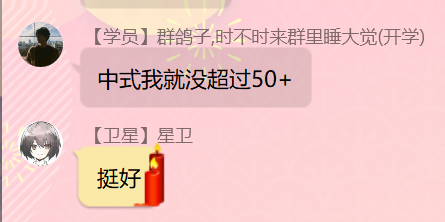
\includegraphics[scale=0.6]{images/1.png}
	\caption{ababababab}
	\label{fig:xiantu}
\end{figure}

\begin{table}[H]
	\begin{tabular}{|rrr|}
		\hline
		直角边 $a$ & 直角边 $b$ & 斜边 $c$ \\
		\hline
		3          & 4          & 5        \\
		5          & 12         & 13       \\
		\hline
	\end{tabular}
	\qquad
	($a^2+b^2=c^2$)
\end{table}


$\angle ACB = \pi / 2$

\section{勾股定理的现代形式}

A-B
ABBR. a\\
汉字abbr\\
\mbox{汉字}abbr

\end{document}